\documentclass[aspectratio=169,11pt]{beamer}

\usepackage{graphicx}
\usepackage{booktabs}
\usepackage{array}
\usepackage{tabularx}
\usepackage{xcolor}
\usepackage{tikz}
\usepackage{listings}
\usepackage{etoolbox}
\usepackage{multimedia}

\setbeamertemplate{navigation symbols}{}
\setbeamertemplate{blocks}[rounded][shadow=true]

\definecolor{oublack}{HTML}{121212}
\definecolor{ougold}{HTML}{B59A57}
\definecolor{ougoldlight}{HTML}{E3D4A5}
\definecolor{oustone}{HTML}{F5F1E8}
\definecolor{ougray}{HTML}{5C5A56}
\definecolor{ouline}{HTML}{D8CCAB}
\definecolor{sbnavy}{HTML}{0E172A}
\definecolor{sbteal}{HTML}{0F766E}
\definecolor{sbsky}{HTML}{38BDF8}
\definecolor{sbcoral}{HTML}{F97316}
\definecolor{sbviolet}{HTML}{7C3AED}
\definecolor{sbgold}{HTML}{F59E0B}
\definecolor{sbmint}{HTML}{EAF7F2}
\definecolor{sbpanel}{HTML}{FBFAF7}
\definecolor{sbtext}{HTML}{1B1A18}
\definecolor{sbmuted}{HTML}{706B63}
\definecolor{sbstring}{HTML}{A5D6FF}
\definecolor{sblight}{HTML}{E6EDF3}

\setbeamercolor{structure}{fg=ougold}
\setbeamercolor{title}{fg=oublack}
\setbeamercolor{subtitle}{fg=ougray}
\setbeamercolor{author}{fg=ougray}
\setbeamercolor{date}{fg=ougray}
\setbeamercolor{normal text}{fg=sbtext,bg=white}
\setbeamercolor{block title}{fg=white,bg=oublack}
\setbeamercolor{block body}{fg=sbtext,bg=sbpanel}
\setbeamercolor{frametitle}{fg=white,bg=oublack}
\setbeamercolor{footline}{fg=white,bg=oublack}

\newcommand{\oaklandwordmarkpath}{images/Oakland_University_logo.png}
\newcommand{\oaklandlogopath}{images/oakland_university_logo-freelogovectors.net_.png}
\newcommand{\oaklandbrandmark}{%
  \IfFileExists{\oaklandlogopath}{%
    \includegraphics[height=0.52cm]{\oaklandlogopath}%
  }{%
    
\begin{tikzpicture}[baseline=(mark.base)]
      \node[rounded corners=3pt, fill=ougold, text=oublack, inner xsep=5pt, inner ysep=2.2pt, font=\scriptsize\bfseries] (mark) {OU};
    \end{tikzpicture}%
  }%
}
\newcommand{\oaklandbrandbadge}{%
  \raisebox{0.275cm}{\tikz[baseline=(box.base)]\node[rounded corners=4pt, fill=oustone, inner xsep=2.2pt, inner ysep=0.2pt] (box) {\oaklandbrandmark};}%
}
\newcommand{\oaklandtitlemark}{%
  \begin{tikzpicture}[baseline=(mark.base)]
    \node[text=white, font=\fontsize{26}{26}\selectfont\bfseries] (mark) {OU};
    \node[text=white!82, font=\fontsize{7.5}{7.5}\selectfont\bfseries] at ([yshift=-10pt]mark.south) {OAKLAND UNIVERSITY};
  \end{tikzpicture}%
}

\setbeamertemplate{background canvas}{%
  \begin{tikzpicture}[remember picture,overlay]
    \fill[white] (current page.south west) rectangle (current page.north east);
    \fill[oustone] (current page.south west) rectangle ([yshift=0.37cm]current page.south east);
    \fill[ougold,opacity=0.10] (-0.8,7.2) circle (2.3);
    \fill[sbteal,opacity=0.05] (13.4,7.4) circle (2.4);
    \fill[ougoldlight,opacity=0.18] (12.7,-0.2) circle (1.7);
    \draw[ouline,line width=0.4pt] ([yshift=0.37cm]current page.south west) -- ([yshift=0.37cm]current page.south east);
  \end{tikzpicture}
}

\setbeamertemplate{frametitle}{%
  \nointerlineskip
  \begin{beamercolorbox}[wd=\paperwidth,ht=1.05cm,dp=0.22cm,leftskip=0.55cm,rightskip=0.3cm]{frametitle}
    
\begin{tikzpicture}[remember picture,overlay]
      \fill[oublack] (0,0) rectangle (\paperwidth,1.28);
      \fill[ougold] (0,0) rectangle (\paperwidth,0.10);
      \fill[ougoldlight,opacity=0.55] (0.55,0.32) rectangle (4.6,0.36);
    \end{tikzpicture}
    \vspace*{0.1cm}\insertframetitle
  \end{beamercolorbox}
}

\setbeamertemplate{footline}{%
  \leavevmode%
  \hbox{%
    \begin{beamercolorbox}[wd=\paperwidth,ht=0.54cm,dp=0.15cm,leftskip=0.38cm,rightskip=0.3cm]{footline}
      \begin{minipage}[c][0.54cm][c]{0.70\paperwidth}
        \centering\raisebox{0.265cm}{\scriptsize\bfseries Oakland University\hspace{0.55em}{\scriptsize School of Engineering and Computer Science}}
      \end{minipage}%
      \begin{minipage}[c][0.54cm][c]{0.14\paperwidth}
        \centering\raisebox{0.265cm}{\scriptsize\insertframenumber/\inserttotalframenumber}
      \end{minipage}%
      \begin{minipage}[c][0.54cm][c]{0.12\paperwidth}
        \centering\oaklandbrandbadge
      \end{minipage}%
    \end{beamercolorbox}%
  }%
}

\lstdefinelanguage{MongoShell}{
  morekeywords={const,db,ObjectId,ISODate,true,false,null},
  morekeywords=[2]{$match,$lookup,$unwind,$project,$group,$sort,$limit,$addFields,$size,$sum,$arrayElemAt,$in,$lte},
  sensitive=true,
  morestring=[b]",
}

\lstdefinestyle{deckquery}{
  language=MongoShell,
  backgroundcolor=\color{sbnavy},
  basicstyle=\ttfamily\fontsize{5.2}{5.8}\selectfont\color{sblight},
  identifierstyle=\color{sblight},
  keywordstyle=\color{sbteal},
  keywordstyle=[2]\color{sbsky},
  stringstyle=\color{sbstring},
  showstringspaces=false,
  breaklines=true,
  columns=fullflexible,
  keepspaces=true,
  frame=single,
  framerule=0pt,
  aboveskip=2pt,
  belowskip=2pt
}

\newcommand{\pill}[2]{%
  \tikz[baseline=-0.6ex]\node[rounded corners=8pt, fill=#1, text=white, inner xsep=8pt, inner ysep=3.5pt, font=\scriptsize\bfseries]{#2};%
}
\newcommand{\ucgoal}[1]{\textcolor{sbteal}{\textbf{Goal:}} #1}
\newcommand{\visualcard}[2]{%
  \begin{beamercolorbox}[wd=\linewidth,rounded=true,shadow=true,sep=0.22cm]{block body}
    \centering
    \includegraphics[width=\linewidth,height=0.57\textheight,keepaspectratio]{#1}
  \end{beamercolorbox}
}
\newcommand{\plainvisual}[2][0.69\textheight]{%
  \centering
  \includegraphics[width=\linewidth,height=#1,keepaspectratio]{#2}
}
\newcommand{\livelyvisual}[1]{%
  \begin{tikzpicture}
    \node[rounded corners=16pt, fill=oustone, minimum width=\linewidth, minimum height=0.66\textheight, inner sep=0pt] (panel) {};
    \fill[sbsky, opacity=0.16] ([xshift=0.35cm,yshift=-0.28cm]panel.north west) circle (0.85cm);
    \fill[sbcoral, opacity=0.14] ([xshift=-0.4cm,yshift=0.35cm]panel.south east) circle (1.0cm);
    \fill[sbteal, opacity=0.10] ([xshift=4.9cm,yshift=-0.2cm]panel.north west) rectangle ++(1.55cm,-0.16cm);
    \node[inner sep=0pt] at (panel.center) {\includegraphics[width=0.95\linewidth,height=0.60\textheight,keepaspectratio]{#1}};
  \end{tikzpicture}%
}
\newcommand{\videocard}[1]{%
  \begin{beamercolorbox}[wd=\linewidth,rounded=true,shadow=true,sep=0.24cm]{block body}
    \centering
    \movie[width=0.92\linewidth,height=0.58\textheight,poster,showcontrols]{}{#1}
  \end{beamercolorbox}
}
\newcommand{\placeholdercard}[1]{%
  \begin{beamercolorbox}[wd=\linewidth,rounded=true,shadow=true,sep=0.22cm]{block body}
    \fbox{%
      \parbox[c][0.57\textheight][c]{0.96\linewidth}{%
        \centering
        \small Screenshot Placeholder\\[0.5em]
        \scriptsize #1
      }%
    }
  \end{beamercolorbox}
}
\setbeamertemplate{title page}{%
  
\begin{tikzpicture}[remember picture,overlay]
    \fill[oustone] (current page.south west) rectangle (current page.north east);
    \fill[ougold] (current page.north west) rectangle ([xshift=3.0cm,yshift=-0.14cm]current page.north west);
    \fill[ougold,opacity=0.12] ([xshift=10.8cm,yshift=5.9cm]current page.south west) circle (2.5cm);
    \fill[sbteal,opacity=0.10] ([xshift=1.0cm,yshift=1.0cm]current page.south west) circle (1.8cm);
    \fill[oublack,opacity=0.05] ([xshift=12.4cm,yshift=1.5cm]current page.south west) circle (1.3cm);
    \draw[ouline,line width=0.7pt] ([xshift=0.62cm,yshift=0.78cm]current page.south west) rectangle ([xshift=-0.62cm,yshift=-0.78cm]current page.north east);
  \end{tikzpicture}
  \vspace*{0.72cm}
  \begin{minipage}[t][0.77\textheight][t]{\textwidth}
    {\color{oublack}\fontsize{21}{25}\selectfont\bfseries\inserttitle\par}
    \vspace{0.45em}
    {\color{sbmuted}\normalsize\insertsubtitle\par}
    \vspace{0.95em}
    {\color{oublack}\normalsize\insertauthor\par}
    \vspace{0.45em}
    {\color{sbmuted}\small School of Engineering and Computer Science\\Computer Science and Engineering Department\par}
    \vspace{0.3em}
    {\color{sbmuted}\small\insertdate\par}
    \vfill
    \IfFileExists{\oaklandwordmarkpath}{%
      \begin{center}
        \includegraphics[width=0.24\linewidth]{\oaklandwordmarkpath}
      \end{center}
    }{%
      \begin{center}
        {\color{oublack}\large Oakland University}
      \end{center}
    }%
  \end{minipage}
}
\title{SkillBridge Final Presentation}
\subtitle{CSI 4999 Senior Capstone Project}
\institute{Oakland University}
\author{Justin Elia \and Spencer Roeren \and Cordell Stonecipher}
\date{Winter 2026}

\begin{document}

\begin{frame}[plain]
  \titlepage
\end{frame}

\begin{frame}{System At A Glance}
  \begin{columns}[T,totalwidth=\textwidth]
    \column{0.30\textwidth}
    \vspace{0.15em}
    {\small SkillBridge turns projects, evidence, resumes, and job analysis into one guided career workspace.}

    \vspace{1.1em}
    \pill{sbteal}{React Frontend}\hspace{0.3em}
    \pill{sbsky}{FastAPI Backend}\hspace{0.3em}
    \pill{sbcoral}{MongoDB}
    \column{0.67\textwidth}
    \plainvisual[0.76\textheight]{images/skillbridge_full_use_case_diagram.png}
  \end{columns}
\end{frame}

\begin{frame}{Users and Core Flows}
  \begin{columns}[T,totalwidth=\textwidth]
    \column{0.49\textwidth}
    {\small\bfseries User Types}\\[-0.15em]
    \begin{columns}[T,totalwidth=\linewidth]
      \column{0.49\linewidth}
      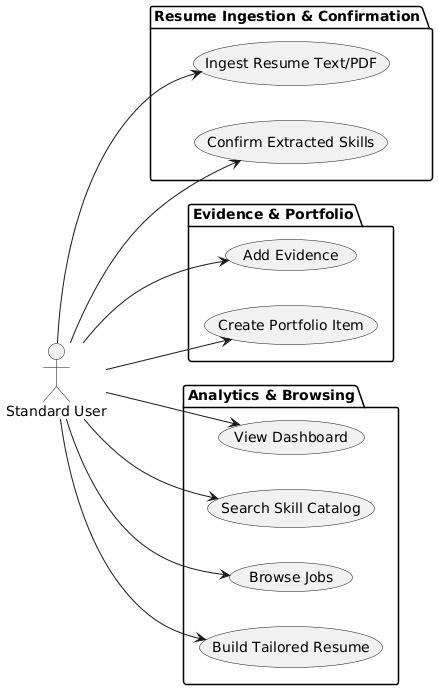
\includegraphics[width=\linewidth,height=0.58\textheight,keepaspectratio,trim=34 22 34 22,clip]{../use_case_standard_user.png}
      \column{0.49\linewidth}
      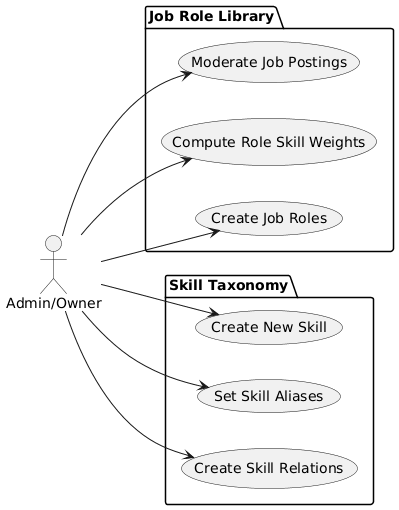
\includegraphics[width=\linewidth,height=0.58\textheight,keepaspectratio,trim=34 22 34 22,clip]{../use_case_admin_user.png}
    \end{columns}
    \column{0.49\textwidth}
    {\small\bfseries Core Pipeline}\\[-0.15em]
    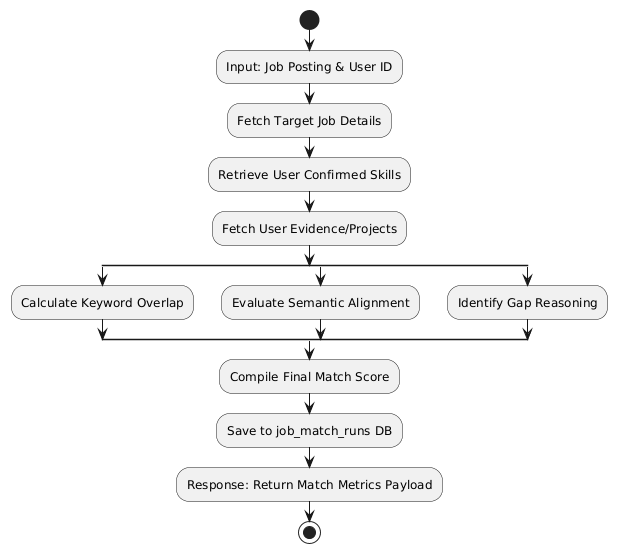
\includegraphics[width=\linewidth,height=0.58\textheight,keepaspectratio,trim=24 28 24 28,clip]{../job_match_analysis_pipeline_flowchart.png}
  \end{columns}
\end{frame}

\begin{frame}{Database ERD}
  \centering
  \resizebox{!}{0.72\textheight}{%
  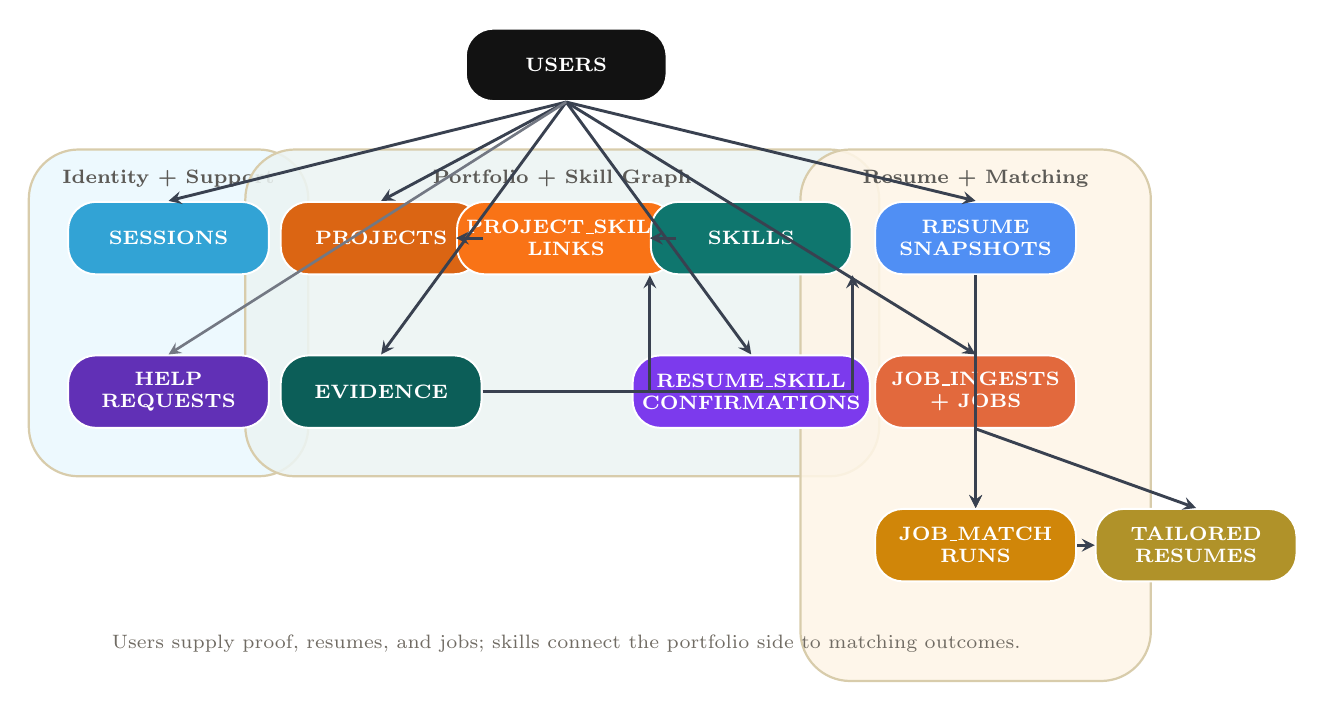
\begin{tikzpicture}[
    x=1cm,y=1cm,
    panel/.style={rounded corners=18pt, draw=ouline, line width=0.8pt, fill=white, fill opacity=0.88, text opacity=1},
    label/.style={font=\scriptsize\bfseries, text=ougray},
    box/.style={rounded corners=10pt, draw=white, line width=0.7pt, text=white, minimum width=2.55cm, minimum height=0.92cm, font=\scriptsize\bfseries, align=center},
    link/.style={draw=sbnavy!82, line width=1.05pt, -stealth},
    softlink/.style={draw=sbnavy!58, line width=0.95pt, -stealth},
    note/.style={font=\scriptsize\color{sbmuted}, align=center}
  ]
    \node[panel, fill=sbsky!10] at (2.3,3.85) [minimum width=3.55cm, minimum height=4.15cm] {};
    \node[label] at (2.3,5.55) {Identity + Support};
    \node[panel, fill=sbteal!8] at (7.3,3.85) [minimum width=8.05cm, minimum height=4.15cm] {};
    \node[label] at (7.3,5.55) {Portfolio + Skill Graph};
    \node[panel, fill=sbgold!10] at (12.55,2.55) [minimum width=4.45cm, minimum height=6.75cm] {};
    \node[label] at (12.55,5.55) {Resume + Matching};

    \node[box, fill=oublack] (users) at (7.35,7.0) {USERS};

    \node[box, fill=sbsky!85!oublack] (sessions) at (2.3,4.8) {SESSIONS};
    \node[box, fill=sbviolet!75!oublack] (help) at (2.3,2.85) {HELP\\REQUESTS};

    \node[box, fill=sbcoral!88!black] (projects) at (5.0,4.8) {PROJECTS};
    \node[box, fill=sbcoral] (links) at (7.35,4.8) {PROJECT\_SKILL\\LINKS};
    \node[box, fill=sbteal] (skills) at (9.7,4.8) {SKILLS};
    \node[box, fill=sbteal!80!black] (evidence) at (5.0,2.85) {EVIDENCE};
    \node[box, fill=sbviolet] (confirm) at (9.7,2.85) {RESUME\_SKILL\\CONFIRMATIONS};

    \node[box, fill=sbsky!65!sbviolet] (resume) at (12.55,4.8) {RESUME\\SNAPSHOTS};
    \node[box, fill=sbcoral!82!sbviolet] (jobs) at (12.55,2.85) {JOB\_INGESTS\\+ JOBS};
    \node[box, fill=sbgold!85!black] (matchruns) at (12.55,0.90) {JOB\_MATCH\\RUNS};
    \node[box, fill=sbgold!70!sbteal] (tailored) at (15.35,0.90) {TAILORED\\RESUMES};

    \draw[link] (users.south) -- (sessions.north);
    \draw[link] (users.south) -- (projects.north);
    \draw[link] (users.south) -- (evidence.north);
    \draw[link] (users.south) -- (confirm.north);
    \draw[link] (users.south) -- (resume.north);
    \draw[link] (users.south) -- (jobs.north);
    \draw[softlink] (users.south) -- (help.north);

    \draw[link] (projects.east) -- (links.west);
    \draw[link] (links.east) -- (skills.west);
    \draw[link] (evidence.east) -| (skills.south west);
    \draw[link] (confirm.west) -| (skills.south east);

    \draw[link] (resume.south) -- (matchruns.north);
    \draw[link] (jobs.south) -- (matchruns.north);
    \draw[link] (jobs.south) -- (tailored.north);
    \draw[link] (matchruns.east) -- (tailored.west);

    \node[note] at (7.35,-0.35) {Users supply proof, resumes, and jobs; skills connect the portfolio side to matching outcomes.};
  \end{tikzpicture}
  }
\end{frame}

\begin{frame}[fragile,shrink=2]{Dashboard Page}
  \begin{columns}[T,totalwidth=\textwidth]
    \column{0.28\textwidth}
    \vspace{-0.7em}
    \begin{block}{Page Coverage}
      {\scriptsize
      \begin{itemize}
        \item UC 1.1 Create / manage project entry
        \item UC 1.4 Dashboard summary
      \end{itemize}
      Dashboard view for portfolio history and progress.}
    \end{block}
    \begin{block}{Mongo Query}
      \begin{lstlisting}[style=deckquery]
db.evidence.aggregate([
  {$match: {user_id: userId}},
  {$unwind: "$skill_ids"},
  {$group: {_id: "$skill_ids",
            evidence_count: {$sum: 1}}}
])
      \end{lstlisting}
    \end{block}
    \column{0.68\textwidth}
    \plainvisual[0.73\textheight]{images/Dashboard.png}
  \end{columns}
\end{frame}

\begin{frame}[fragile]{Evidence Page}
  \begin{columns}[T,totalwidth=\textwidth]
    \column{0.28\textwidth}
    \vspace{-0.25em}
    \begin{block}{Page Coverage}
      {\scriptsize
      \begin{itemize}
        \item UC 1.3 Add evidence and associate it
      \end{itemize}
      Proof capture, extraction, and save workflow.}
    \end{block}
    \begin{block}{Mongo Query}
      \begin{lstlisting}[style=deckquery]
db.evidence.findOne(
  {_id: ObjectId("69c487ec4f7976837a6b2402")},
  {title: 1, type: 1,
   project_id: 1, skill_ids: 1}
)
      \end{lstlisting}
    \end{block}
    \column{0.68\textwidth}
    \plainvisual[0.75\textheight]{images/pr5_add_evidence_frontend.png.png.png}
  \end{columns}
\end{frame}

\begin{frame}[fragile,shrink=5]{Skills}
  \begin{columns}[T,totalwidth=\textwidth]
    \column{0.28\textwidth}
    \vspace{-0.45em}
    \begin{block}{Page Coverage}
      {\scriptsize
      \begin{itemize}
        \item UC 2.1 Add a skill with category and tags
        \item UC 2.2 Update skill proficiency
        \item UC 2.4 Skill gap analysis
      \end{itemize}
      Main profile skill-management page.}
    \end{block}
    \begin{block}{Mongo Query}
      \begin{lstlisting}[style=deckquery]
db.resume_skill_confirmations.findOne(
  {user_id: userId,
   resume_snapshot_id: null},
  {confirmed: {$slice: 3},
   updated_at: 1}
)
      \end{lstlisting}
    \end{block}
    \column{0.68\textwidth}
    \visualcard{images/Skills.png}{One page for confirmed skills, proficiency control, and profile-facing skill management.}
  \end{columns}
\end{frame}

\begin{frame}[fragile,shrink=5]{Skill Detail View}
  \begin{columns}[T,totalwidth=\textwidth]
    \column{0.28\textwidth}
    \vspace{-0.45em}
    \begin{block}{Page Coverage}
      {\scriptsize
      \begin{itemize}
        \item UC 1.2 Link a skill to a project
        \item UC 2.3 View skill detail with linked evidence
      \end{itemize}
      One skill tied to proof and project context.}
    \end{block}
    \begin{block}{Mongo Query}
      \begin{lstlisting}[style=deckquery]
db.project_skill_links.aggregate([
  {$match: {skill_id: skillId}},
  {$lookup: {from: "projects",
             localField: "project_id",
             foreignField: "_id",
             as: "project"}}
])
      \end{lstlisting}
    \end{block}
    \column{0.68\textwidth}
    \visualcard{images/week6_skill_detail.png}{Expanded skill detail page connecting one skill to proof and project context.}
  \end{columns}
\end{frame}

\begin{frame}[fragile,shrink=5]{Resume Workflow}
  \begin{columns}[T,totalwidth=\textwidth]
    \column{0.28\textwidth}
    \vspace{-0.45em}
    \begin{block}{Page Coverage}
      {\scriptsize
      \begin{itemize}
        \item UC 3.1 Resume ingestion
        \item UC 3.2 Skill extraction
        \item UC 3.3 Confirm / reject / edit extracted skills
        \item UC 3.4 Persist confirmed skills to the profile
      \end{itemize}
      Resume-to-profile skill pipeline.}
    \end{block}
    \begin{block}{Mongo Query}
      \begin{lstlisting}[style=deckquery]
db.resume_skill_confirmations.findOne(
  {_id: ObjectId("69a1df28994bc3fc6cd4751c")},
  {confirmed: 1, rejected: 1, edited: 1}
)
      \end{lstlisting}
    \end{block}
    \column{0.68\textwidth}
    \visualcard{../ssdconfirmedextractedskills.png}{The confirmation screen shows extraction review, correction, and final promotion into the user's profile.}
  \end{columns}
\end{frame}

\begin{frame}[fragile,shrink=5]{Admin Job Review}
  \begin{columns}[T,totalwidth=\textwidth]
    \column{0.28\textwidth}
    \vspace{-0.45em}
    \begin{block}{Admin moderation and job intelligence}
      {\scriptsize
      \begin{itemize}
        \item UC 4.1 Review and moderate submitted jobs
        \item UC 4.2 Tag a posting by role
        \item UC 4.3 Aggregate postings by role
      \end{itemize}}
    \end{block}
    \begin{block}{Mongo Query}
      \begin{lstlisting}[style=deckquery]
db.jobs.findOne(
  {_id: ObjectId("69cd6a8856c9b08e2ae488c4")},
  {title: 1, company: 1,
   moderation_status: 1,
   role_ids: 1}
)
      \end{lstlisting}
    \end{block}
    \column{0.68\textwidth}
    \visualcard{images/week6_admin_job_review.png}{One admin page for moderation decisions, role tagging, and reusable job review data.}
  \end{columns}
\end{frame}

\begin{frame}[fragile]{Taxonomy}
  \begin{columns}[T,totalwidth=\textwidth]
    \column{0.28\textwidth}
    \begin{block}{Alias and relationship maintenance}
      {\scriptsize
      \begin{itemize}
        \item UC 4.4 Maintain taxonomy
      \end{itemize}}
    \end{block}
    \begin{block}{Mongo Query}
      \begin{lstlisting}[style=deckquery]
db.skill_relations.aggregate([
  {$match: {$or: [
    {from_skill_id: skillId},
    {to_skill_id: skillId}
  ]}}
])
      \end{lstlisting}
    \end{block}
    \column{0.68\textwidth}
    \visualcard{images/week6_skill_relations.png}{Taxonomy editing page for skill aliases and relationship maintenance.}
  \end{columns}
\end{frame}

\begin{frame}[fragile]{Jobs Page}
  \begin{columns}[T,totalwidth=\textwidth]
    \column{0.28\textwidth}
    \begin{block}{Page Coverage}
      {\scriptsize
      \begin{itemize}
        \item AF 1 Generate job-match analysis
        \item AF 2 Generate and save tailored resumes
      \end{itemize}
      Job fit and resume customization page.}
    \end{block}
    \begin{block}{Mongo Query}
      \begin{lstlisting}[style=deckquery]
db.job_match_runs.find(
  {user_id: userId}
).sort({created_at: -1}).limit(3)
      \end{lstlisting}
    \end{block}
    \column{0.68\textwidth}
    \livelyvisual{../ssdanalyzejobmatch.png}
  \end{columns}
\end{frame}

\begin{frame}[fragile]{Analytics and Help Pages}
  \begin{columns}[T,totalwidth=\textwidth]
    \column{0.28\textwidth}
    \begin{block}{Page Coverage}
      {\scriptsize
      \begin{itemize}
        \item AF 3 Skill analytics, learning paths, career paths
        \item AF 4 Help requests and admin responses
      \end{itemize}
      Guidance and support pages.}
    \end{block}
    \begin{block}{Mongo Query}
      \begin{lstlisting}[style=deckquery]
db.help_requests.find(
  {user_id: userId}
).sort({created_at: -1})
      \end{lstlisting}
    \end{block}
    \column{0.68\textwidth}
    \placeholdercard{Insert current Skill Analytics screenshot and Help page screenshot side by side or as a stitched export.}
  \end{columns}
\end{frame}

\begin{frame}{Project Demo Video}
  \begin{center}
    \IfFileExists{videos/final_presentation_demo.mp4}{%
      \videocard{videos/final_presentation_demo.mp4}
    }{%
      \placeholdercard{Drop the presentation demo at \texttt{reports/videos/final\_presentation\_demo.mp4} and this slide will embed it automatically.}
    }%
  \end{center}
\end{frame}

\begin{frame}{Thank You}
  \begin{columns}[T,totalwidth=\textwidth]
    \column{0.62\textwidth}
    {\Large\bfseries Thank you for your time.}

    \vspace{0.9em}
    {\small
    This presentation covered the final SkillBridge product, including 20 implemented use cases, the Mongo-backed data model, and the full user-to-admin workflow across skills, evidence, resumes, jobs, analytics, and help.}
    \column{0.34\textwidth}
    \begin{center}
      \vspace{1.4em}
      {\Huge \textbf{Any Questions?}}
    \end{center}
  \end{columns}
\end{frame}

\end{document}
